\documentclass{assignment}

\course{ECO 120-04}
\name{Lucas Reddinger}
\date{Friday 9 December 2022}
\doctitle{Assignment 10 Solutions}

\begin{document}
\RaggedRight

\beginsolutions{}

Suppose that the U.S.~economy is initially in long-run equilibrium, producing its potential output $Y_P$, as depicted directly below.

\begin{tikzpicture}[scale=0.6]
\draw[thick,<->] (0,10) node[below left,label={[align=right]left:Aggregate\\price level\\ }] {$P$} --(0,0)--(18,0) node[below left,label=right:Real GDP]{$Y$};
\draw[very thick,blue] (1,6.5) --(12,1) node[right]{$\text{AD}_1$};
\draw[very thick,orange] (9,0) node[below]{$Y_P$}--(9,8) node[above]{LRAS};
\draw[very thick,red] (7,1)--(15,7) node[right]{$\text{SRAS}_1$};
\draw[dashed] (0,2.5) node[left]{$P^*_1$} --(9,2.5) ;
\end{tikzpicture}

A multinational effort to sanction Russian oil and natural gas results in a negative shock to short-run aggregate supply from $\text{SRAS}_1$ to $\text{SRAS}_2$ as depicted below. U.S.~economic output falls from $Y_P$ to $Y^*_2$, and the aggregate price level rises from $P^*_1$ to $P^*_2$. This results in a period of \emph{stagflation}---lower economic output coupled with inflation.

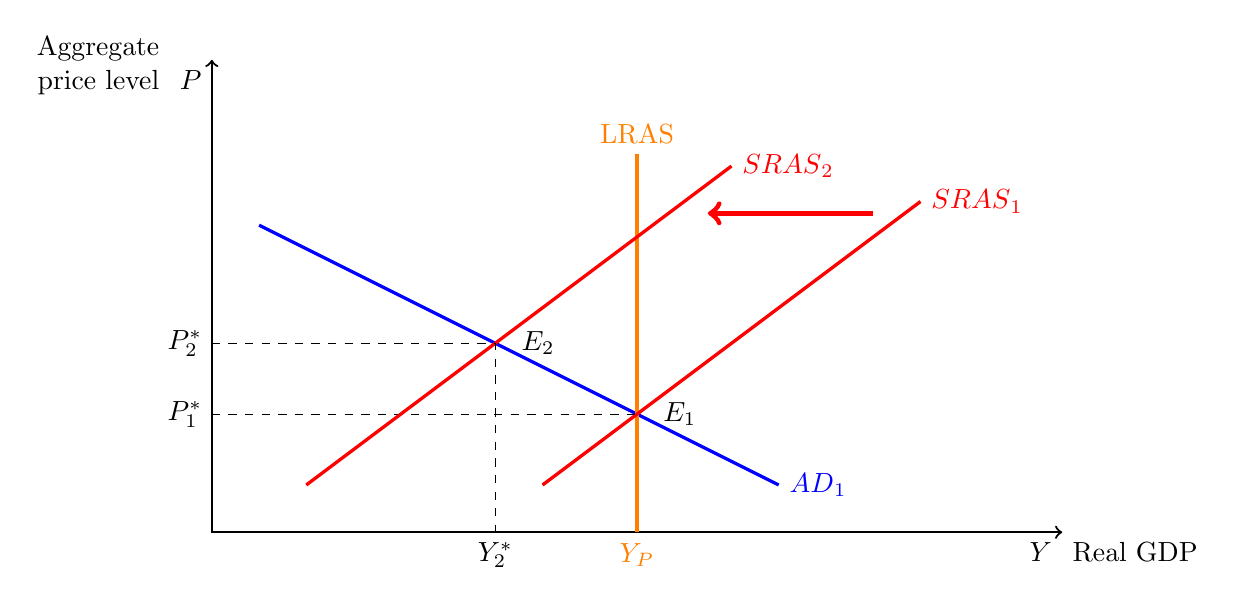
\begin{tikzpicture}[scale=0.6]
\draw[thick,<->] (0,10) node[below left,label={[align=right]left:Aggregate\\price level\\ }] {$P$} --(0,0)--(18,0) node[below left,label=right:Real GDP]{$Y$};
\draw[very thick,blue] (1,6.5) --(12,1) node[right]{$\text{AD}_1$};
\draw[very thick,orange] (9,0) node[below]{$Y_P$}--(9,8) node[above]{LRAS};
\draw[very thick,red] (7,1)--(15,7) node[right]{$\text{SRAS}_1$};
\draw[dashed] (0,2.5) node[left]{$P^*_1$} --(9,2.5) node[right,xshift=6pt]{$E_1$};
\draw[very thick,red] (2,1) --(11,7.75) node[right]{$\text{SRAS}_2$};
\draw[dashed] (0,4) node[left]{$P^*_2$} --(6,4) node[right,xshift=6pt]{$E_2$} --(6,0)node[below]{$Y^*_2$};
\draw[line width=2pt,->,red] (14,6.75)--(10.5,6.75);
\end{tikzpicture}


\begin{enumerate}

\item \label{maintain-output} Please illustrate how fiscal policy could be used to maintain economic growth. \\ {\footnotesize Hint: Reproduce the second graph here. Illustrate a change in fiscal policy that restores output to $Y_P$.}

\begin{solution}
To maintain economic growth, we would want to achieve actual output equal to potential output. Thus we would want to shift the AD curve until $Y_P$ is achieved with $\text{SRAS}_2$.

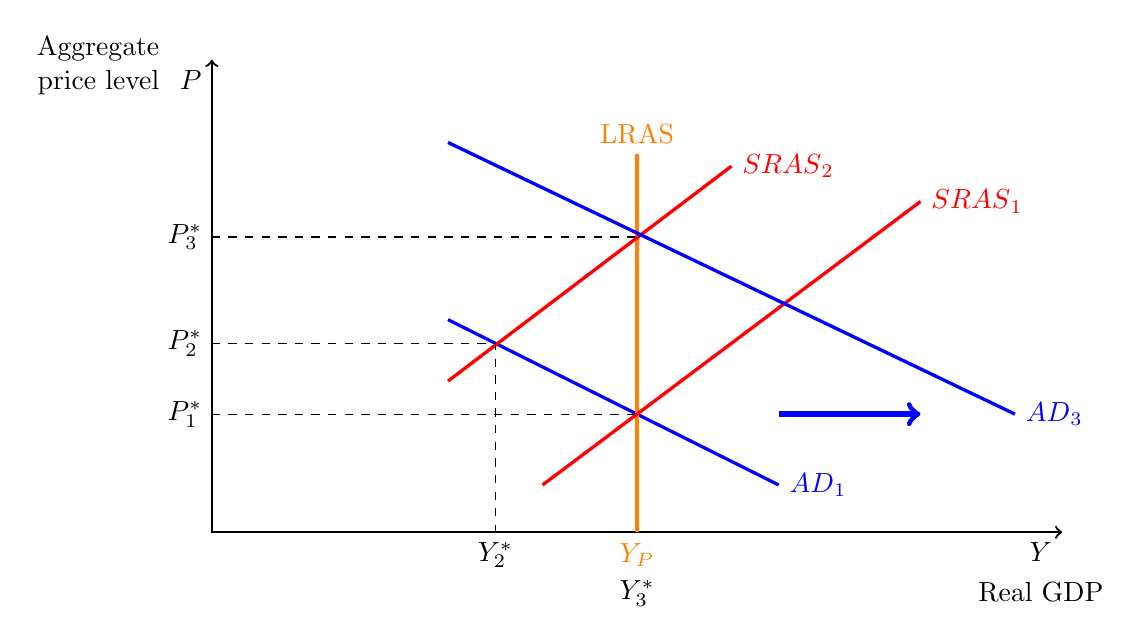
\begin{tikzpicture}[scale=0.6]
\draw[thick,<->] (0,10) node[below left,label={[align=right]left:Aggregate\\price level\\ }] {$P$} --(0,0)--(18,0) node[below left,label=below:Real GDP]{$Y$};
\draw[very thick,blue] (5,4.5)--(12,1) node[right]{$\text{AD}_1$};
\draw[very thick,orange] (9,0) node[below]{$Y_P$}--(9,8) node[above]{LRAS};
\draw[very thick,red] (7,1)--(15,7) node[right]{$\text{SRAS}_1$};
\draw[dashed] (0,2.5) node[left]{$P^*_1$}--(9,2.5) node[right,xshift=6pt]{};
\draw[very thick,red] (5,3.2)--(11,7.75) node[right]{$\text{SRAS}_2$};
\draw[dashed] (0,4) node[left]{$P^*_2$}--(6,4) node[right,xshift=6pt]{} --(6,0)node[below]{$Y^*_2$};

\draw[very thick,blue] (5,8.25)--(17,2.5) node[right]{$\text{AD}_3$};
\draw[dashed] (0,6.25) node[left]{$P^*_3$}--(9,6.25) node[right,xshift=6pt]{};
\node[below,yshift=-14pt] at (9,0) {$Y^*_3$};

\draw[line width=2pt,->,blue] (12,2.5)--(15,2.5);
\end{tikzpicture}
\end{solution}

\item \label{maintain-prices} Please illustrate how fiscal policy could be used to stabilize prices. \\ {\footnotesize Hint: Reproduce the second graph here. Illustrate a change in fiscal policy that restores the price level to $P^*_1$.}

\begin{solution}
To stabilize the price level, we would want to achieve P equal to $P^*_1$. Thus we would want to shift the AD curve until $P^*_1$ is achieved with $\text{SRAS}_2$.

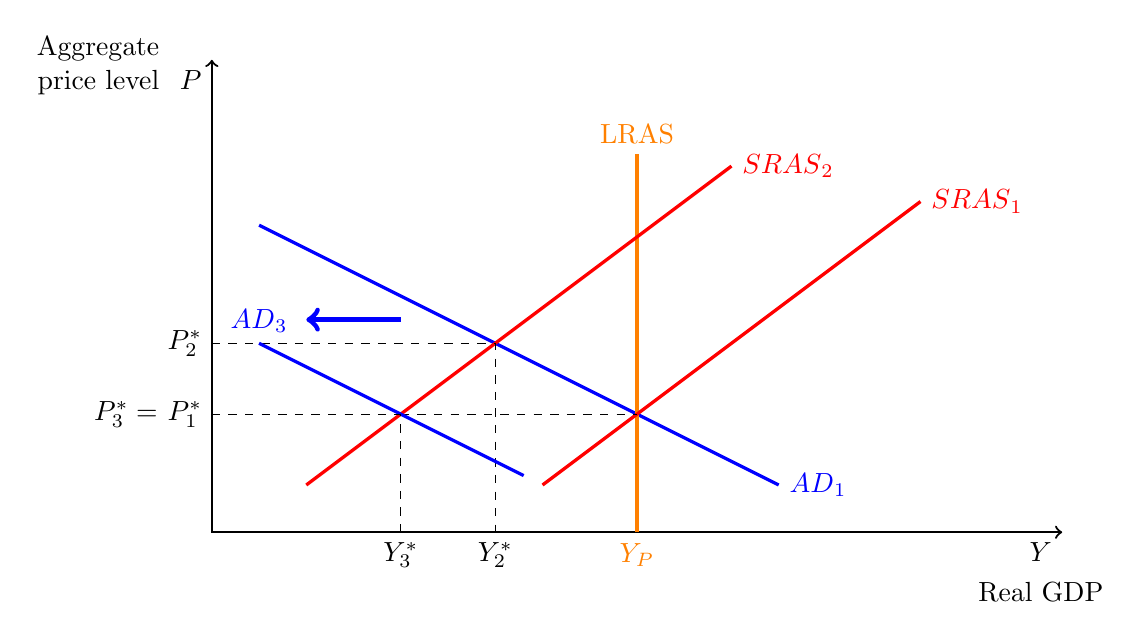
\begin{tikzpicture}[scale=0.6]
\draw[thick,<->] (0,10) node[below left,label={[align=right]left:Aggregate\\price level\\ }] {$P$} --(0,0)--(18,0) node[below left,label=below:Real GDP]{$Y$};
\draw[very thick,blue] (1,6.5) --(12,1) node[right]{$\text{AD}_1$};
\draw[very thick,orange] (9,0) node[below]{$Y_P$}--(9,8) node[above]{LRAS};
\draw[very thick,red] (7,1)--(15,7) node[right]{$\text{SRAS}_1$};
\draw[dashed] (4,2.5) --(9,2.5) node[right,xshift=6pt]{};
\draw[very thick,red] (2,1) --(11,7.75) node[right]{$\text{SRAS}_2$};
\draw[dashed] (0,4) node[left]{$P^*_2$} --(6,4) node[right,xshift=6pt]{} --(6,0)node[below]{$Y^*_2$};

\draw[very thick,blue] (1,4) node[above]{$\text{AD}_3$} --(6.6,1.2);
\draw[dashed] (0,2.5) node[left,xshift=-16pt]{$P^*_3=$} --(4,2.5) node[above,xshift=-1pt]{} --(4,0) node[below]{$Y^*_3$};
\node[left] at (0,2.5) {$P^*_1$};

\draw[line width=2pt,->,blue] (4,4.5)--(2,4.5);
\end{tikzpicture}
\end{solution}

\item Can fiscal policy remedy stagflation? Please explain with a complete sentence.  \\ {\footnotesize Hint: Can a change in fiscal policy restore \emph{both} output to $Y_P$ \emph{and} the price level to $P^*_1$?}

\begin{solution}
Stagflation refers to output stagnation coupled with inflation. We see stagflation at $E_2$ relative to $E_1$ because $Y^*_2<Y_P$ (output is decreased) and $P^*_2>P^*_1$ (the price level is increased).

In \cref{maintain-output}, the proposed policy restores economic output ($Y^*_3=Y_P$), but it worsens inflation ($P^*_3 \gg P^*_1$). In \cref{maintain-prices}, the proposed policy restores the price level ($P^*_3=P^*_1$), but it further depresses output ($Y^*_3 \ll Y_P$).

We conclude that by shifting the aggregate demand curve, higher output can be achieved (but with higher prices) or lower prices can be achieved (but with lower inflation).

A shift of the aggregate demand curve \emph{cannot both} lower the price level and \emph{also} raise output.
\end{solution}

\end{enumerate}

\end{document}
